\begin{frame}{Encoder-Decoder Architecture}
  \begin{itemize}
    \item[\textcolor{red}{$\blacktriangleright$}] \textbf{Encoder:} Stack of self-attention and feed-forward (FF) layers.
    \item[\textcolor{red}{$\blacktriangleright$}] \textbf{Decoder:} Adds masked self-attention and encoder-decoder attention on top of FF layers.
    \item[\textcolor{red}{$\blacktriangleright$}] \textbf{Applications:} Widely used in tasks like translation, summarization, and more.
  \end{itemize}
\end{frame}

\begin{frame}{Encoder}
  \centering
  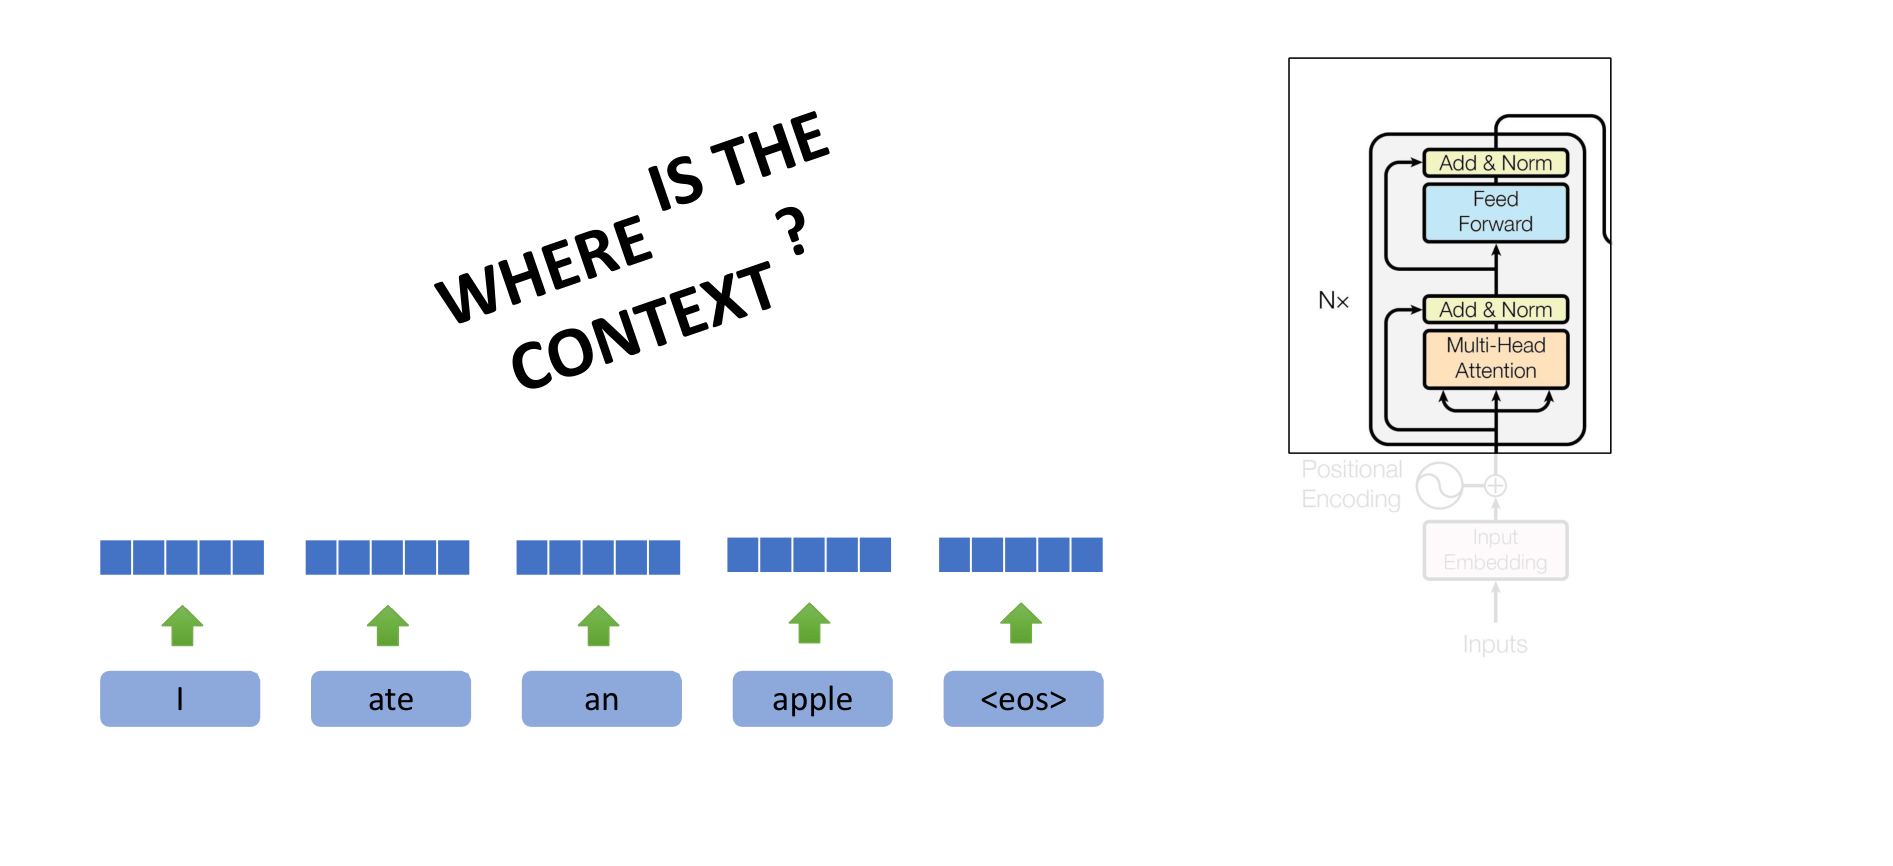
\includegraphics[width=\paperwidth,height=0.95\paperheight,keepaspectratio]{images/introduction-to-transformers/transformer_block_where_is_the_context.png}
\end{frame}

\begin{frame}{Encoder}
  \centering
  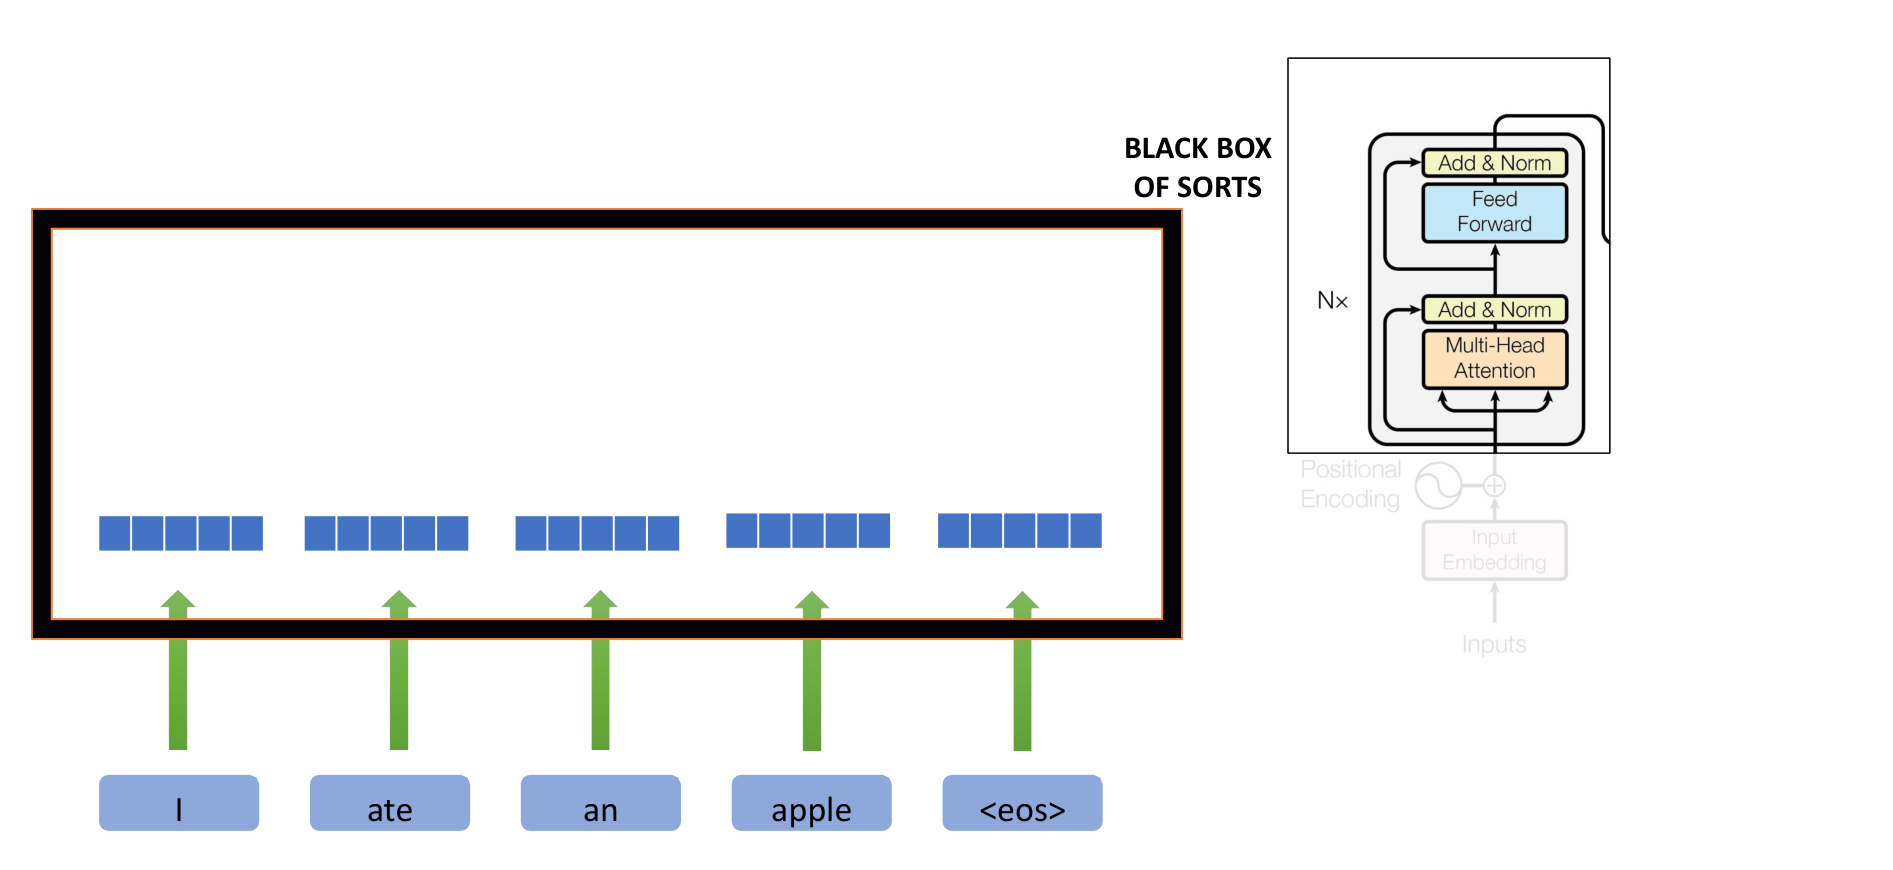
\includegraphics[width=\paperwidth,height=0.95\paperheight,keepaspectratio]{images/introduction-to-transformers/transformer_block_black_box_of_sorts.png}
\end{frame}

\begin{frame}{Encoder}
  \centering
  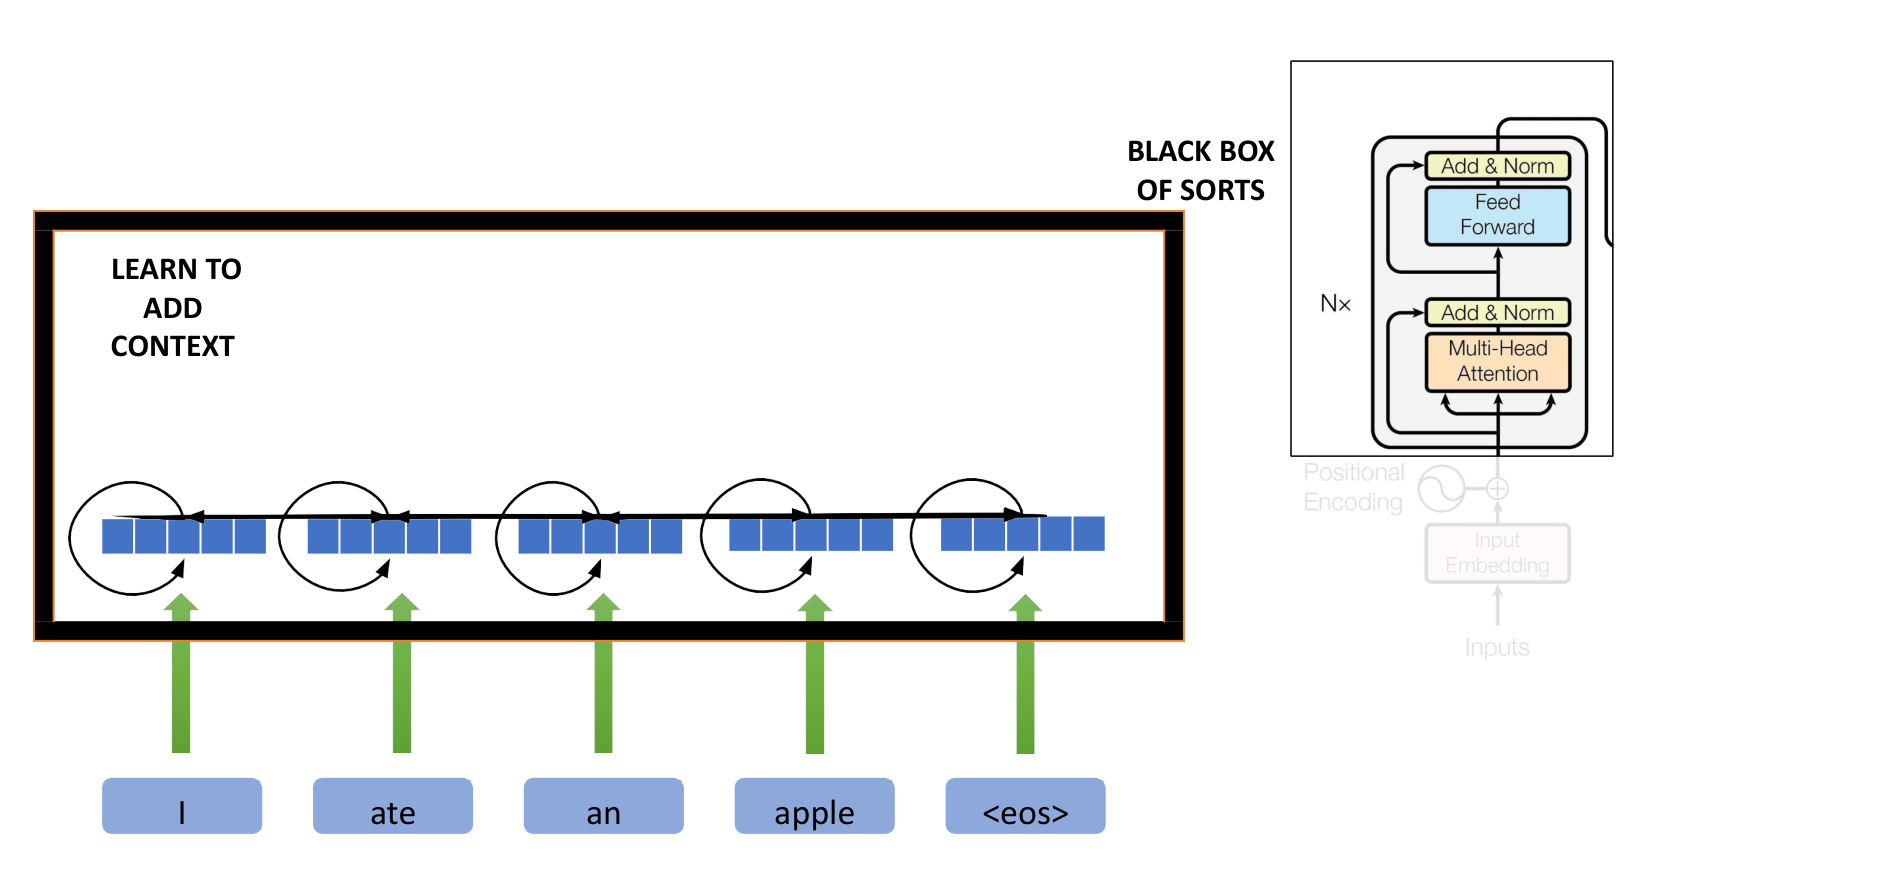
\includegraphics[width=\paperwidth,height=0.95\paperheight,keepaspectratio]{images/introduction-to-transformers/transformer_block_learn_to_add_context.png}
\end{frame}

\begin{frame}{Encoder}
  \centering
  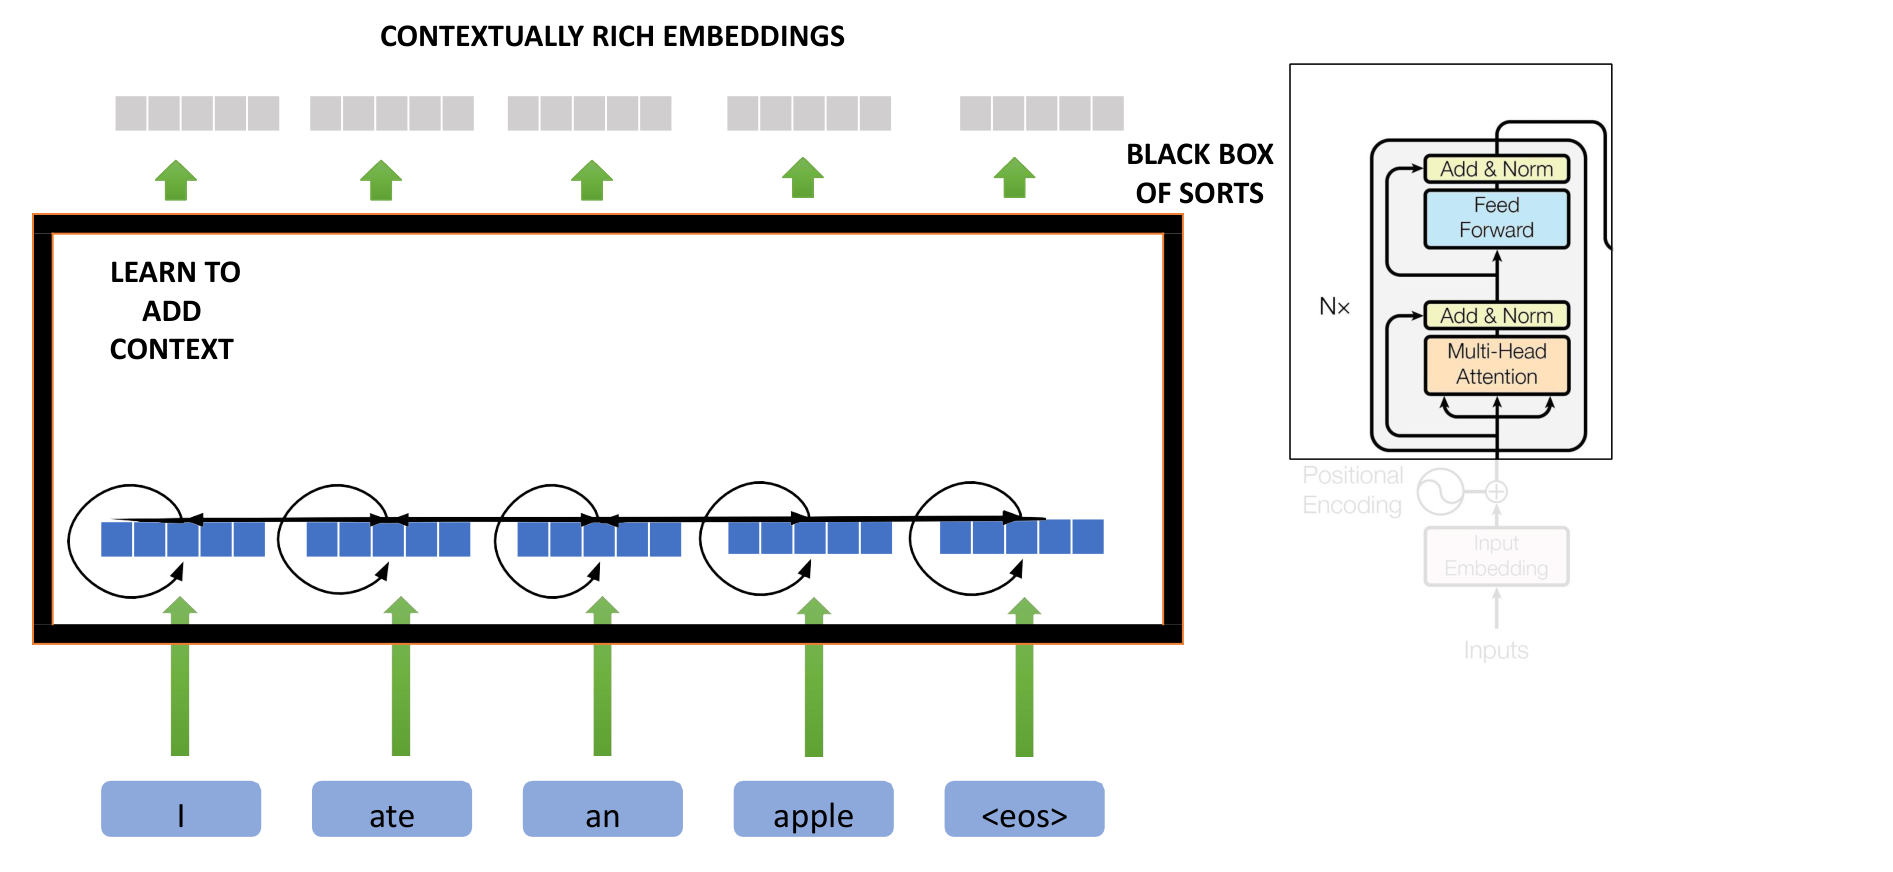
\includegraphics[width=\paperwidth,height=0.95\paperheight,keepaspectratio]{images/introduction-to-transformers/transformer_block_contextually_rich_embeddings.png}
\end{frame}

\begin{frame}{Encoder}
  \centering
  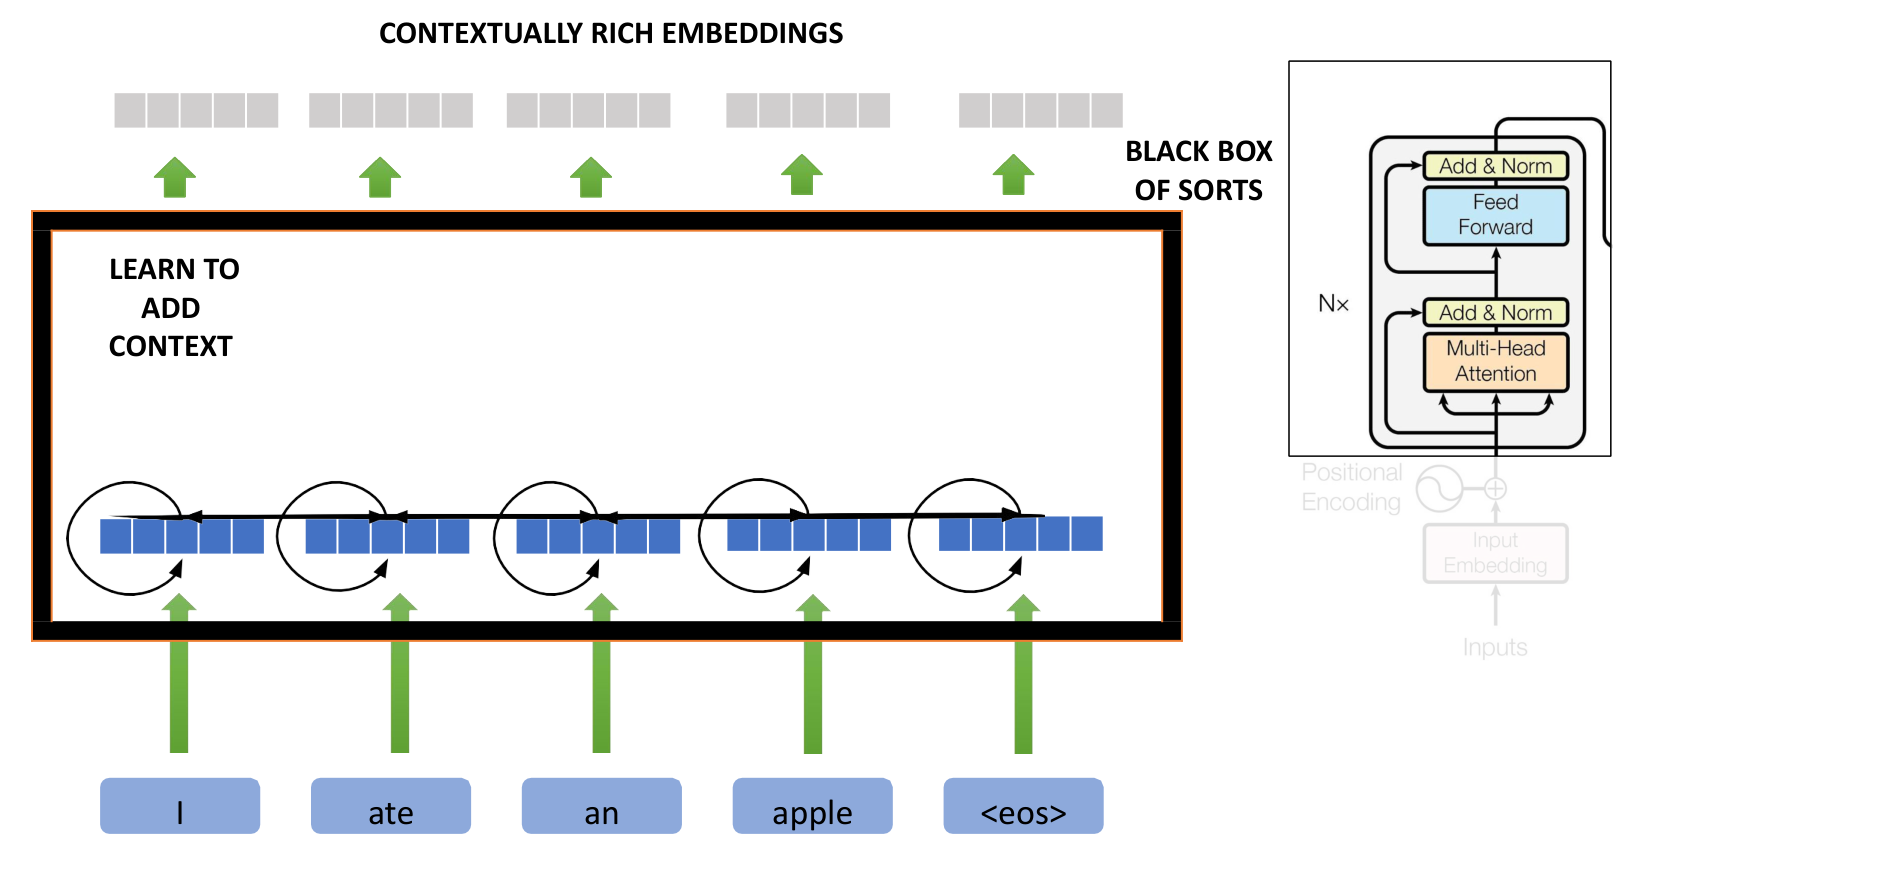
\includegraphics[width=\paperwidth,height=0.95\paperheight,keepaspectratio]{images/introduction-to-transformers/transformer_block_contextually_rich_embeddings_highlighted.png}
\end{frame}

\begin{frame}{Encoder-Only Transformers}
  \begin{itemize}
    \item[\textcolor{red}{$\blacktriangleright$}] \textbf{Example:} BERT
    \item[\textcolor{red}{$\blacktriangleright$}] Only the encoder stack is used.
    \item[\textcolor{red}{$\blacktriangleright$}] \textbf{Applications:} Classification, question answering, embeddings.
  \end{itemize}
\end{frame}

\begin{frame}{Encoders}
  \centering
  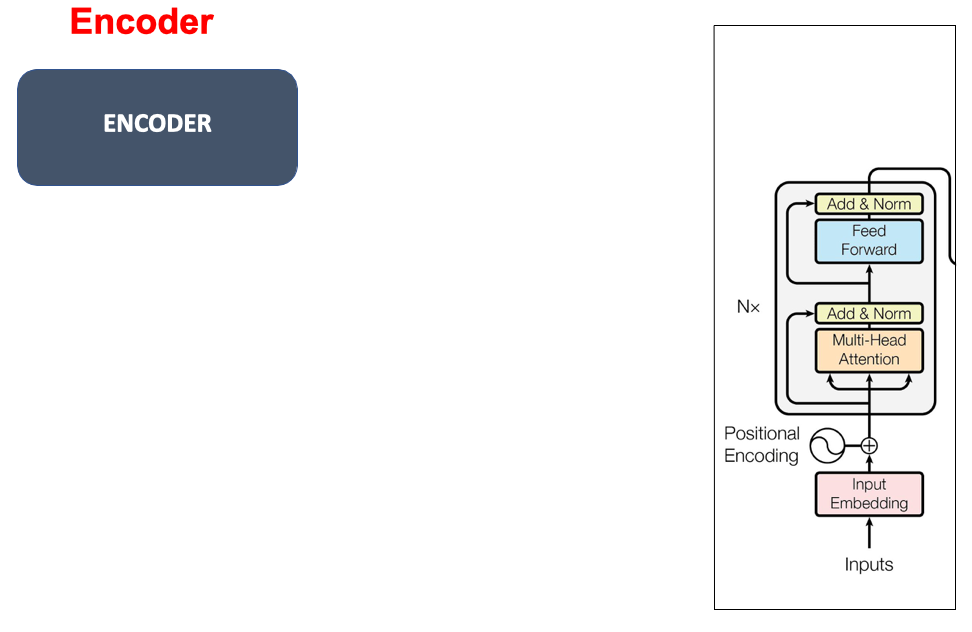
\includegraphics[width=0.8\paperwidth,height=0.8\paperheight,keepaspectratio]{images/introduction-to-transformers/transformer_encoder_single_block_highlight.png}
\end{frame}

\begin{frame}{Encoders}
  \centering
  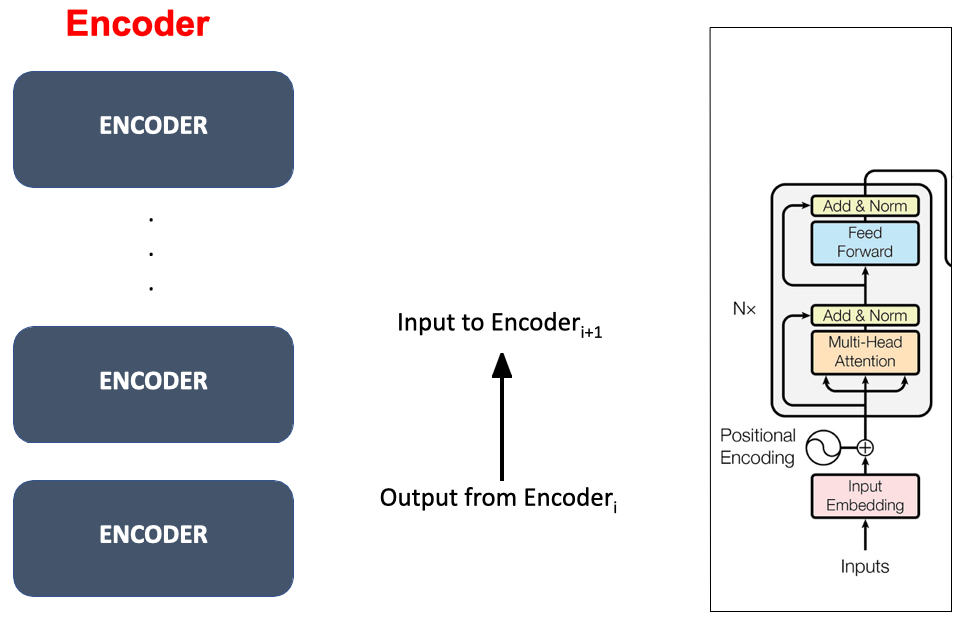
\includegraphics[width=0.8\paperwidth,height=0.8\paperheight,keepaspectratio]{images/introduction-to-transformers/transformer_encoder_stack_output_to_next_input.png}
\end{frame}

\begin{frame}{Encoder-Decoder Attention}
  \centering
  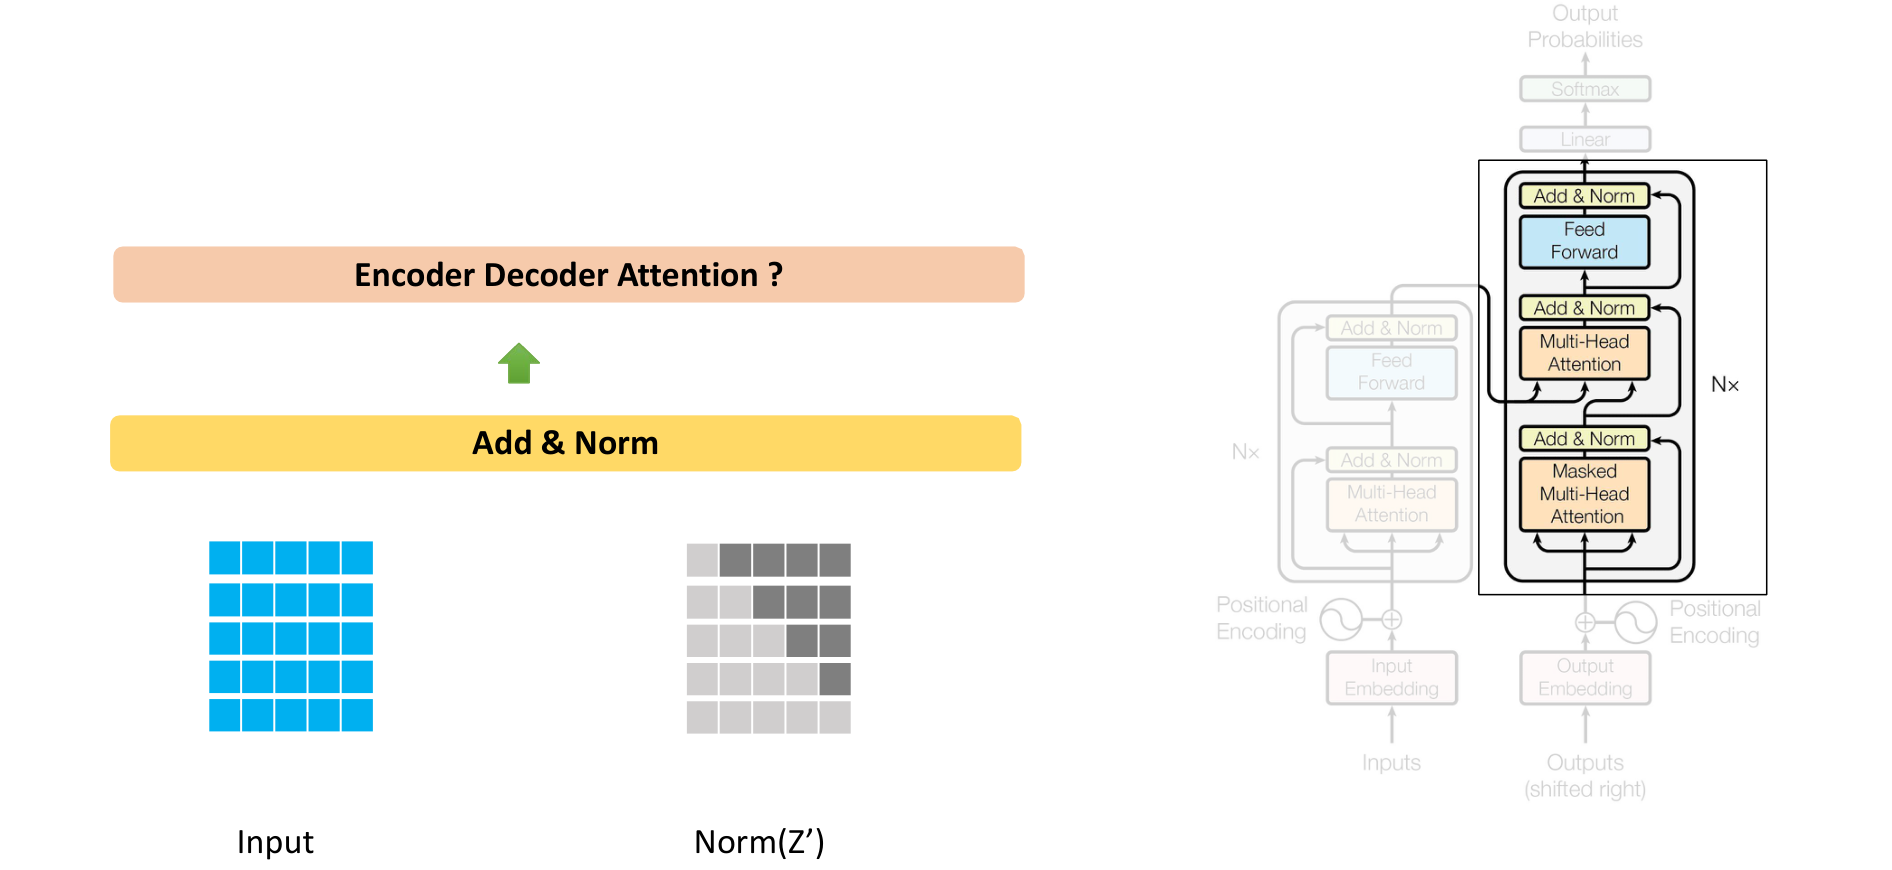
\includegraphics[width=0.9\paperwidth,height=0.9\paperheight,keepaspectratio]{images/introduction-to-transformers/transformer_encoder_decoder_attention_add_norm_input.png}
\end{frame}

\begin{frame}{Encoder-Decoder Attention}
  \centering
    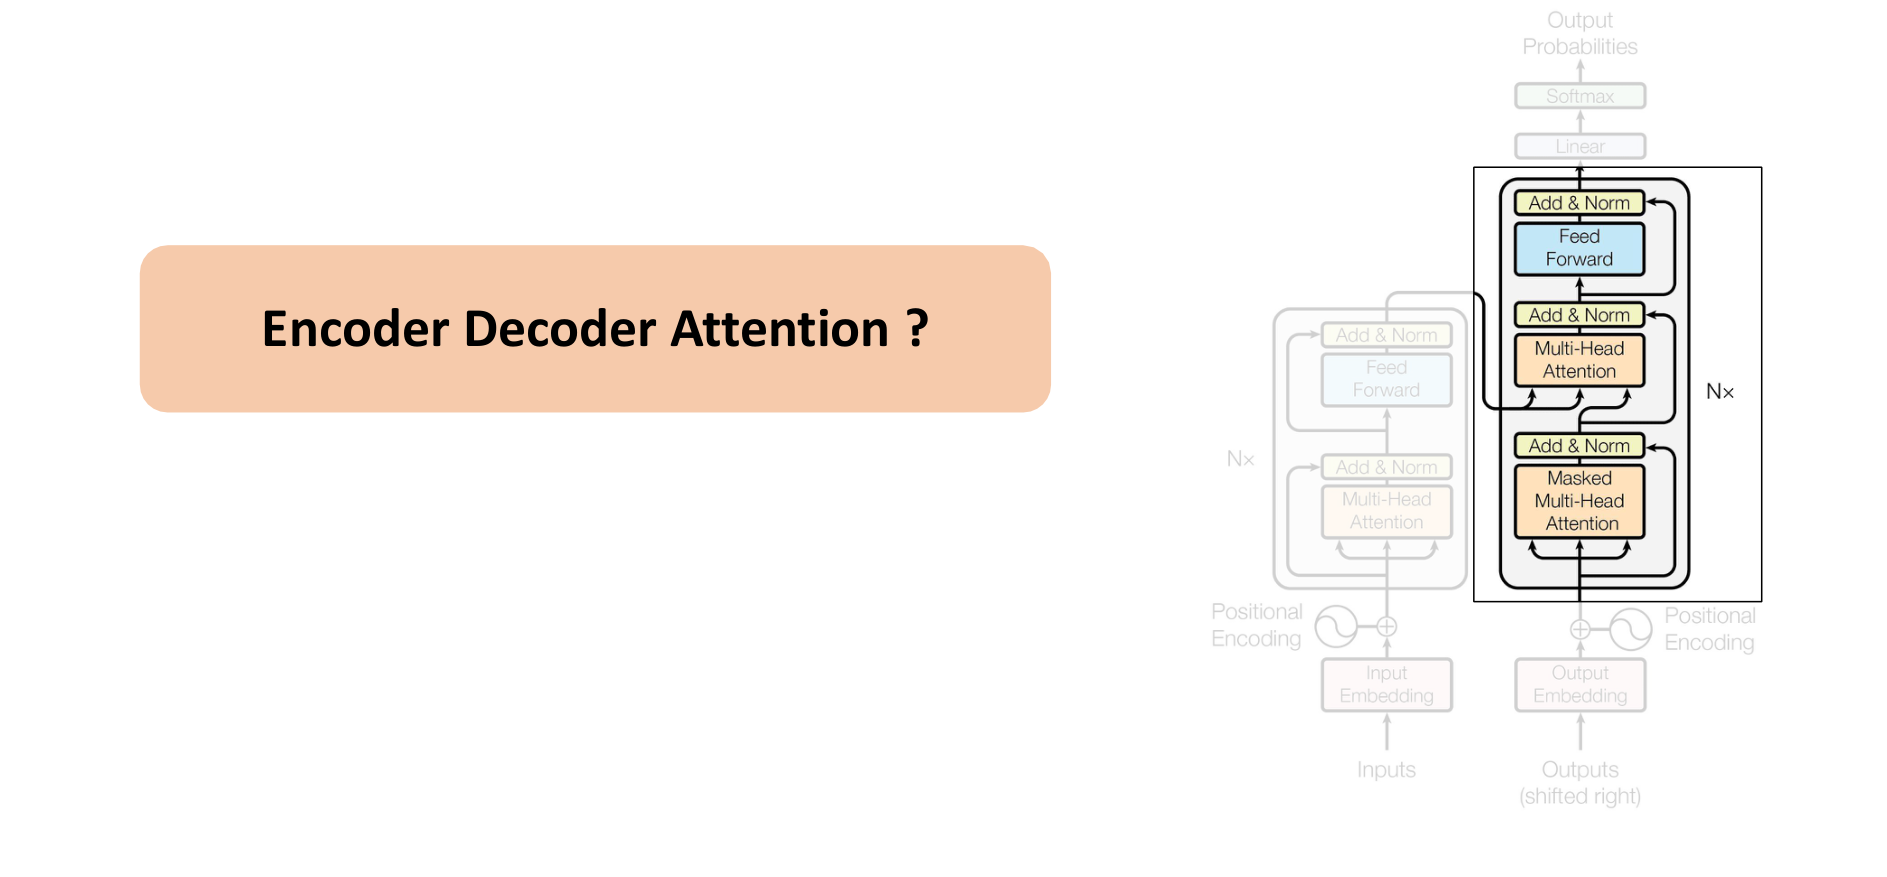
\includegraphics[width=0.9\paperwidth,height=0.9\paperheight,keepaspectratio]{images/introduction-to-transformers/transformer_encoder_decoder_attention_decoder_highlight.png}
\end{frame}

\begin{frame}{Encoder-Decoder Attention}
  \centering
  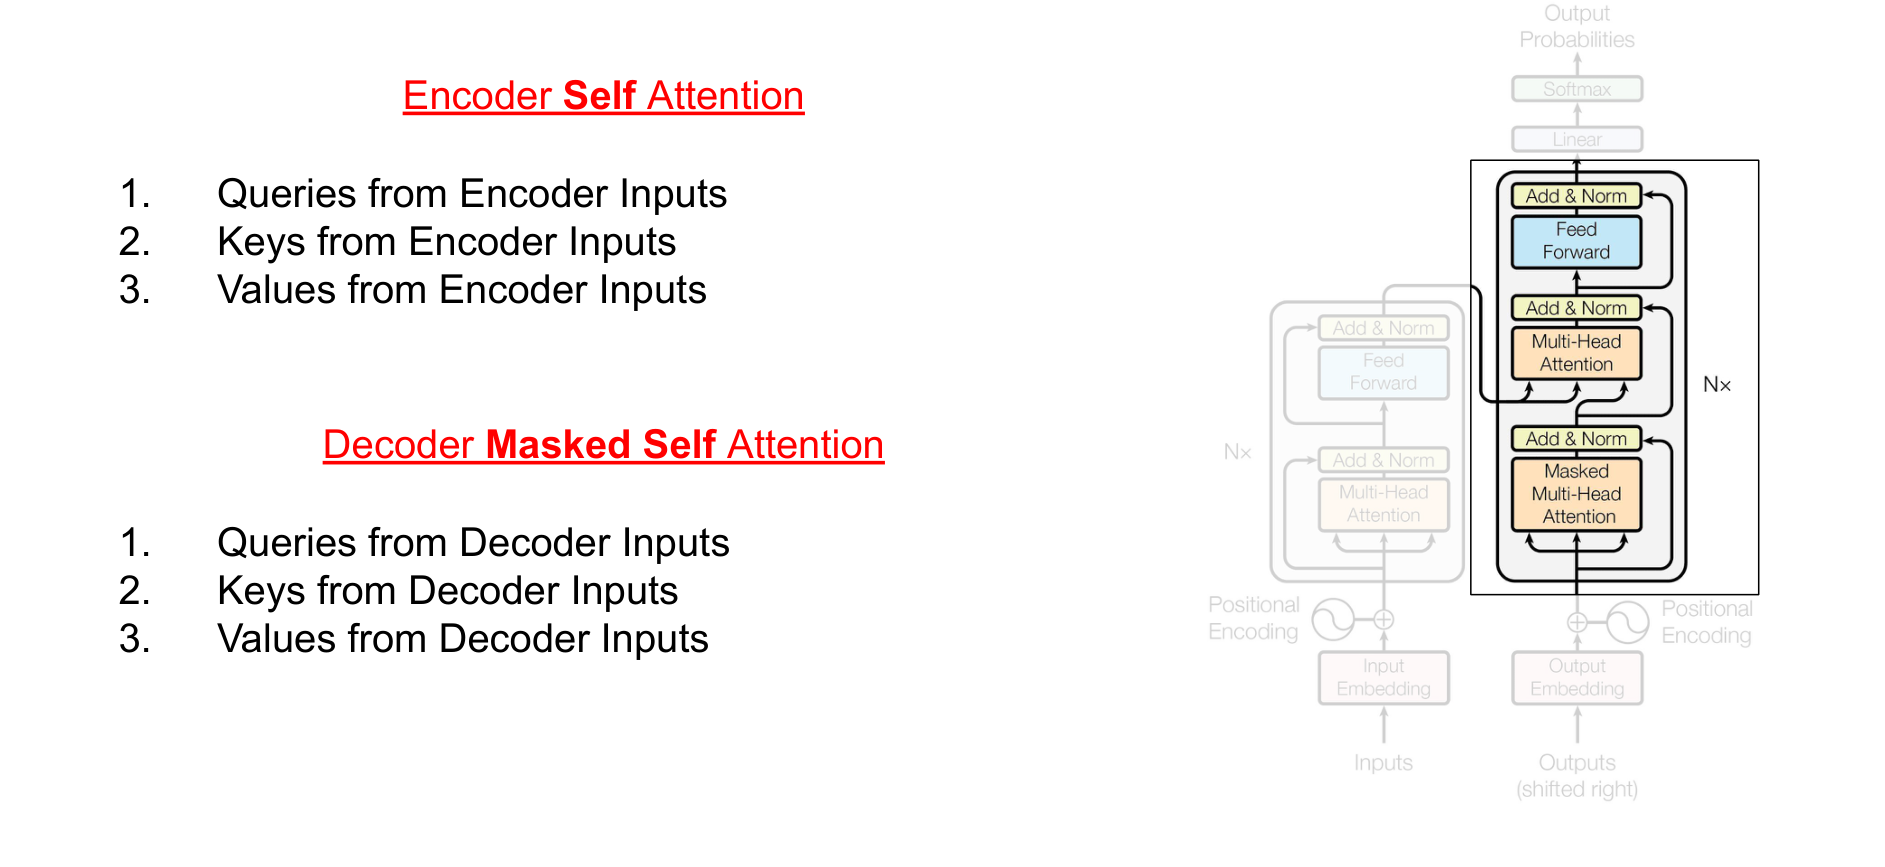
\includegraphics[width=0.9\paperwidth,height=0.9\paperheight,keepaspectratio]{images/introduction-to-transformers/transformer_encoder_self_vs_decoder_masked_self_attention.png} 
\end{frame}

\begin{frame}{Encoder-Decoder Attention}
  \centering
  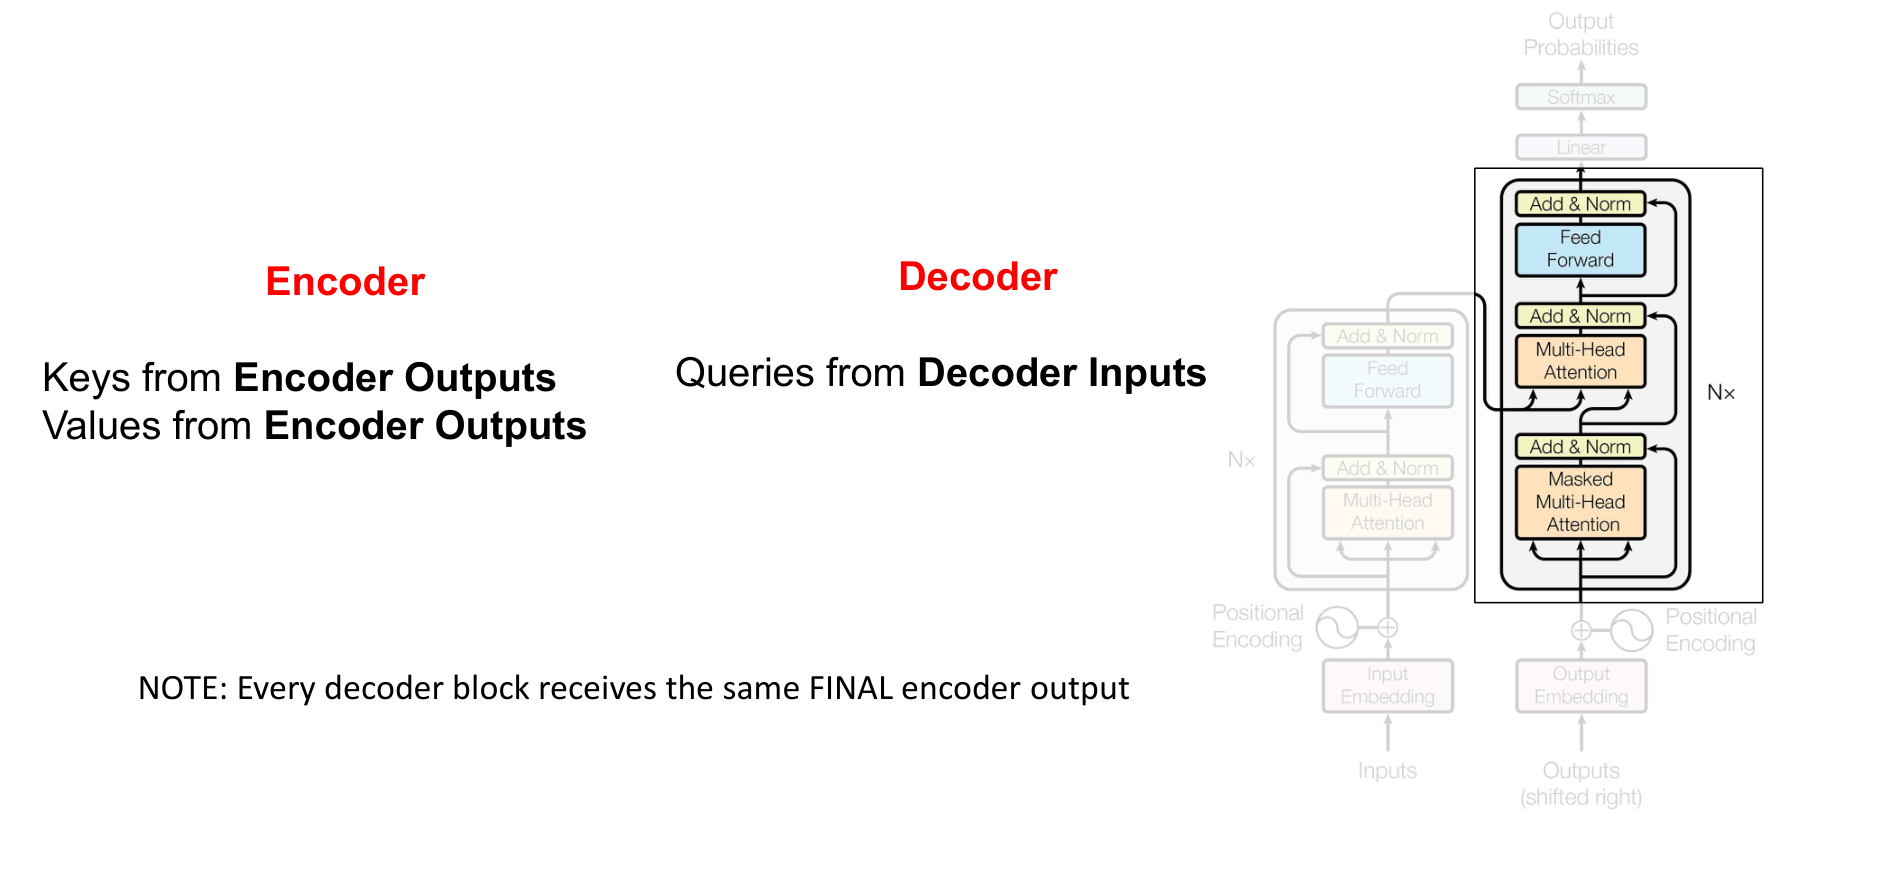
\includegraphics[width=0.9\paperwidth,height=0.9\paperheight,keepaspectratio]{images/introduction-to-transformers/transformer_cross_attention_encoder_keys_values_decoder_queries.png}
\end{frame}

\begin{frame}{Encoder-Decoder Attention}
  \centering
  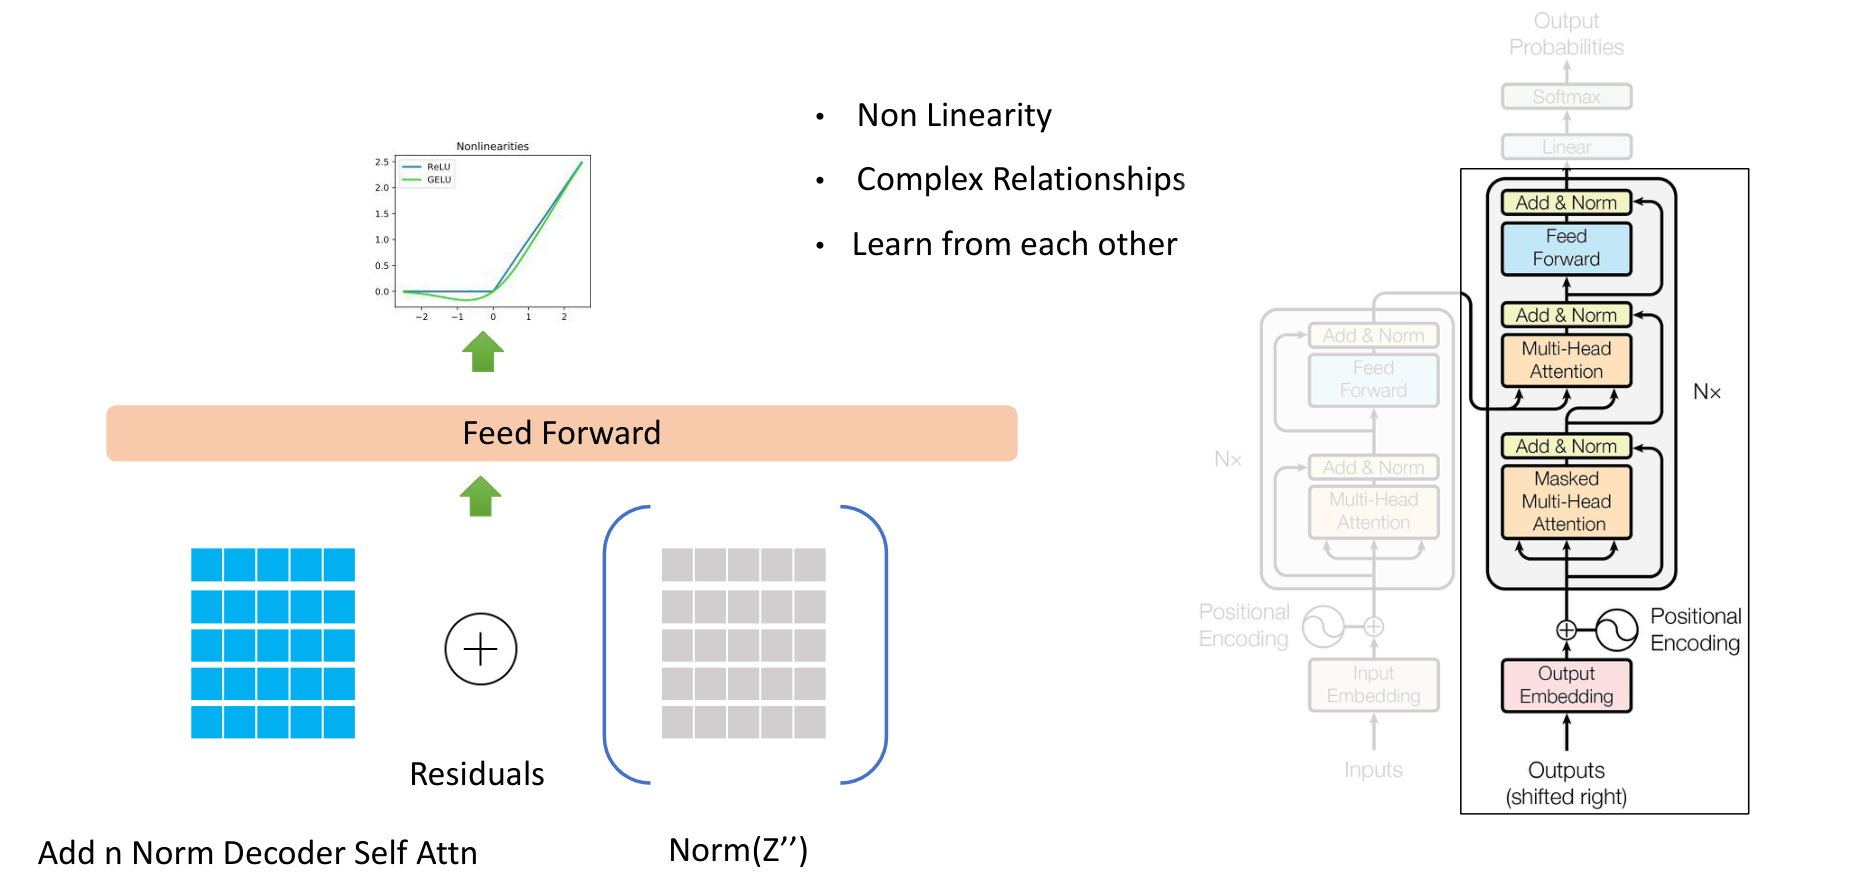
\includegraphics[width=0.9\paperwidth,height=0.9\paperheight,keepaspectratio]{images/introduction-to-transformers/transformer_decoder_feed_forward_nonlinearity_residuals.png}
\end{frame}

\begin{frame}{Decoder-Only Transformers}
  \begin{itemize}
    \item[\textcolor{red}{$\blacktriangleright$}] \textbf{Example:} GPT, LLaMA
    \item[\textcolor{red}{$\blacktriangleright$}] Uses only the decoder block.
    \item[\textcolor{red}{$\blacktriangleright$}] \textbf{Masked self-attention (causal):} Each token can only attend to previous tokens.
    \item[\textcolor{red}{$\blacktriangleright$}] \textbf{Applications:} Language modeling, text generation.
  \end{itemize}
\end{frame}

\begin{frame}{Decoder}
  \centering
  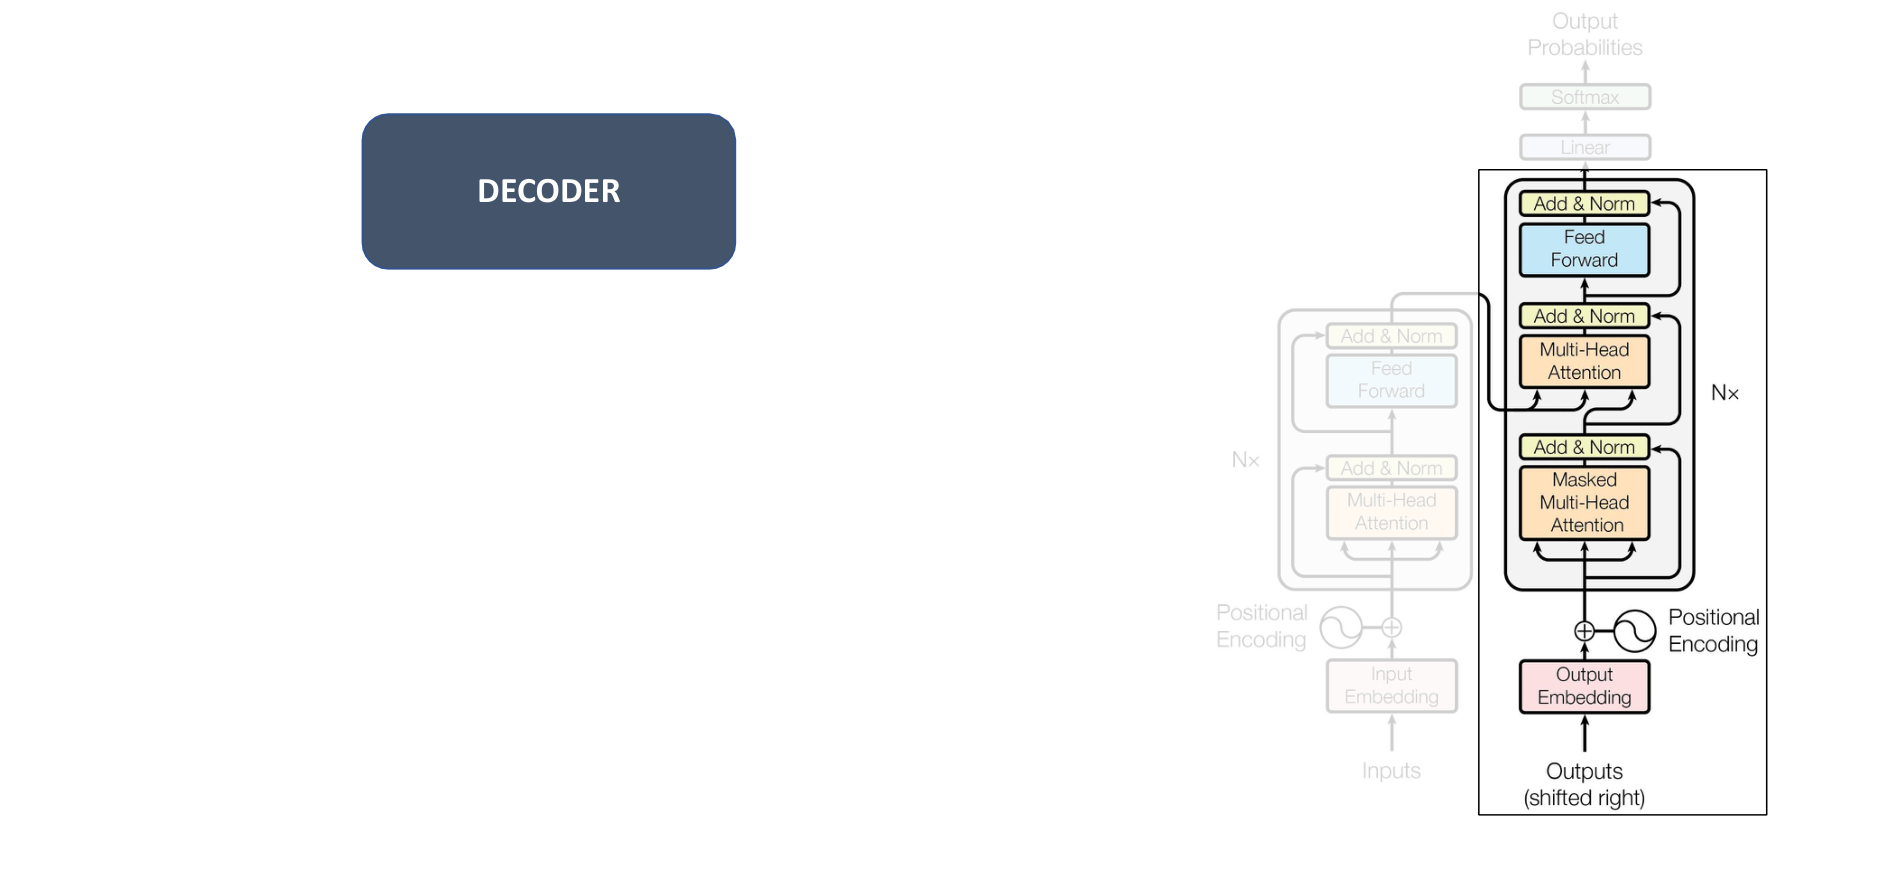
\includegraphics[width=0.8\paperwidth,height=0.8\paperheight,keepaspectratio]{images/introduction-to-transformers/transformer_decoder_block_highlighted.png}
\end{frame}

\begin{frame}{Decoder}
  \centering
  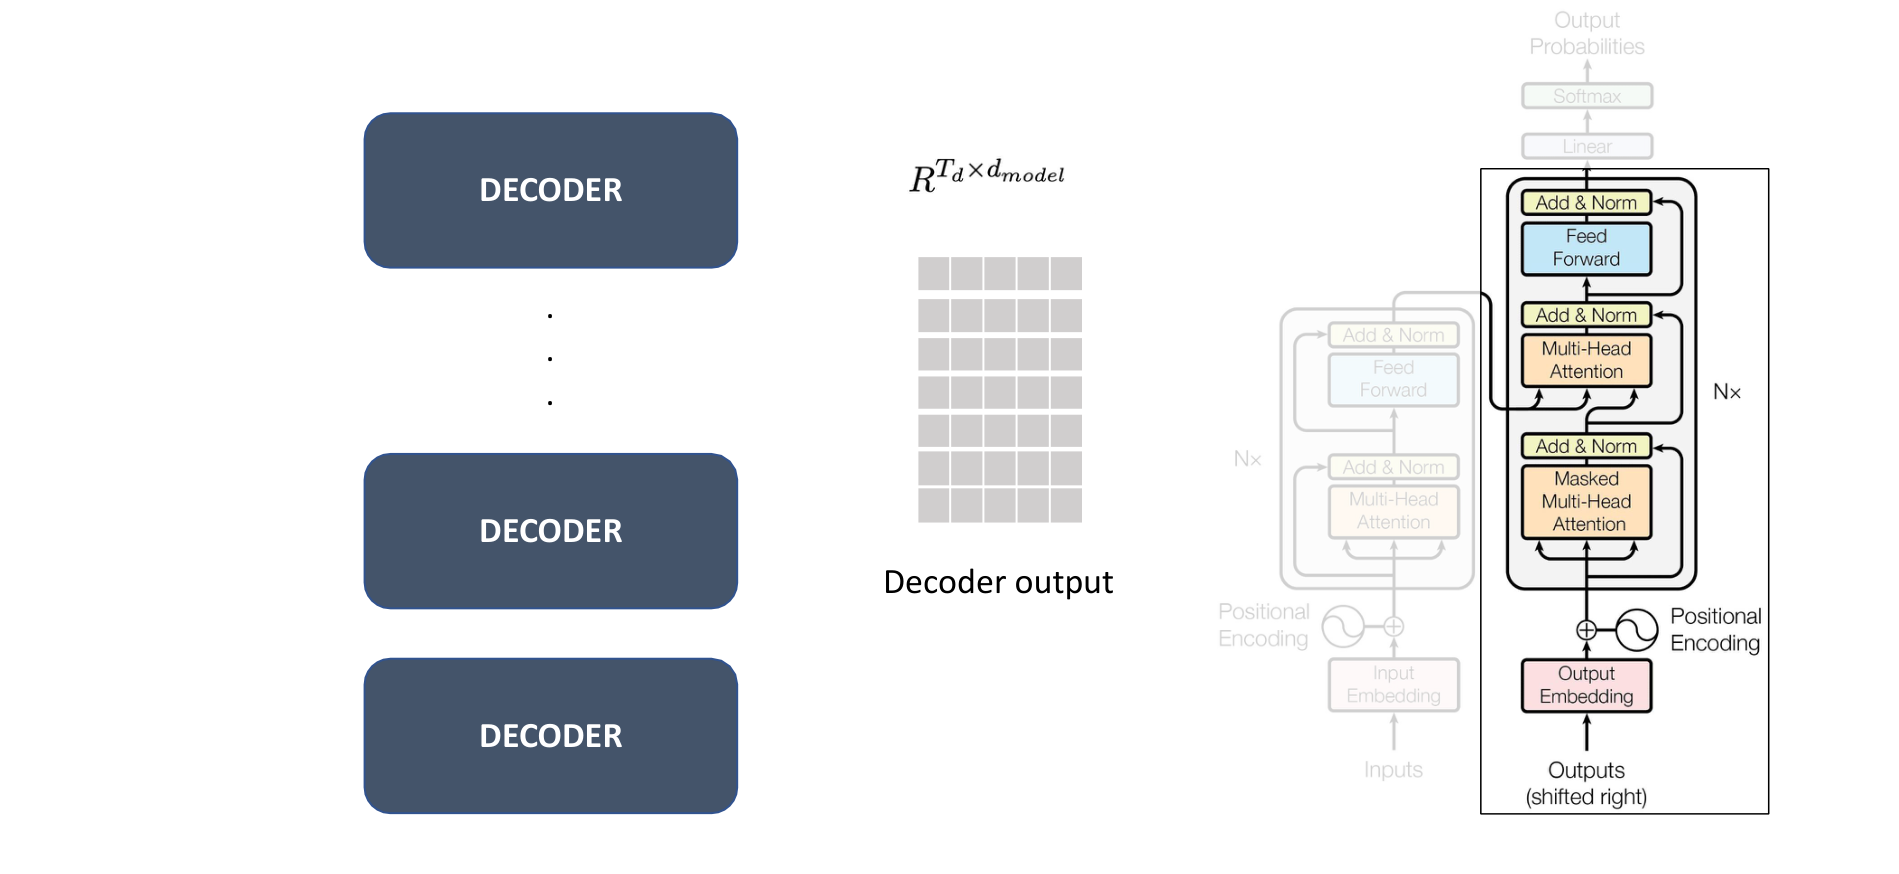
\includegraphics[width=0.8\paperwidth,height=0.8\paperheight,keepaspectratio]{images/introduction-to-transformers/transformer_decoder_stack_output_matrix.png}
\end{frame}

\begin{frame}{Linear}
  \centering
  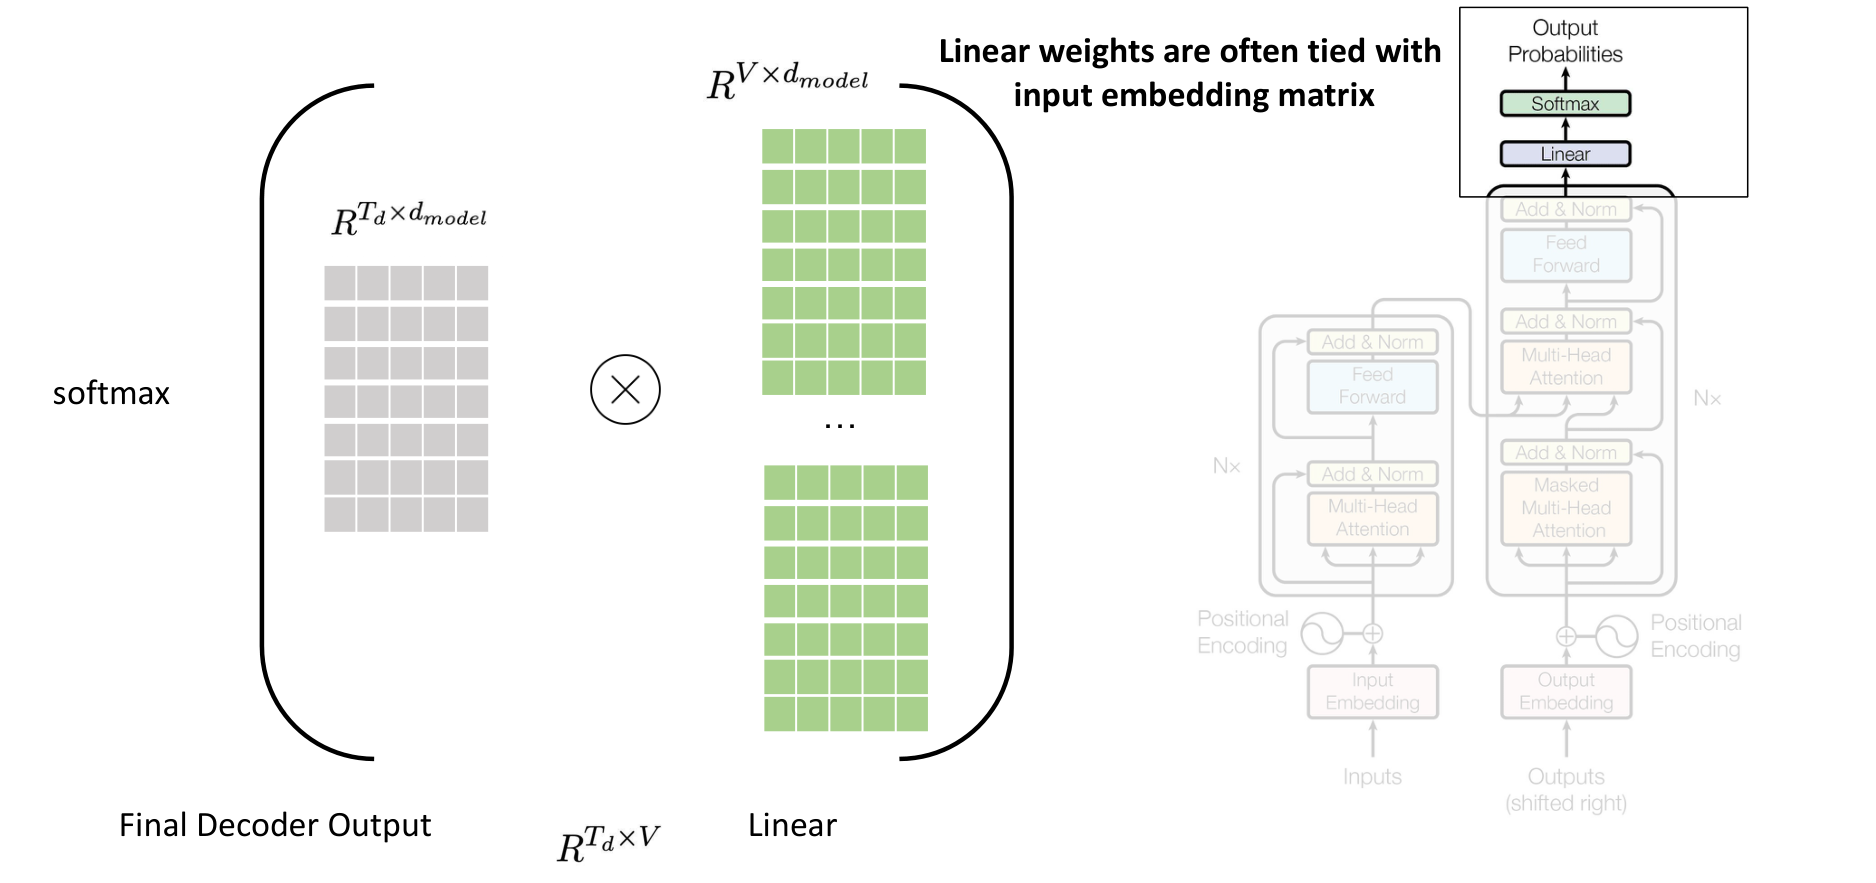
\includegraphics[width=0.8\paperwidth,height=0.8\paperheight,keepaspectratio]{images/introduction-to-transformers/transformer_linear_projection_tied_embedding_weights.png}
\end{frame}

\begin{frame}{Softmax}
  \centering
  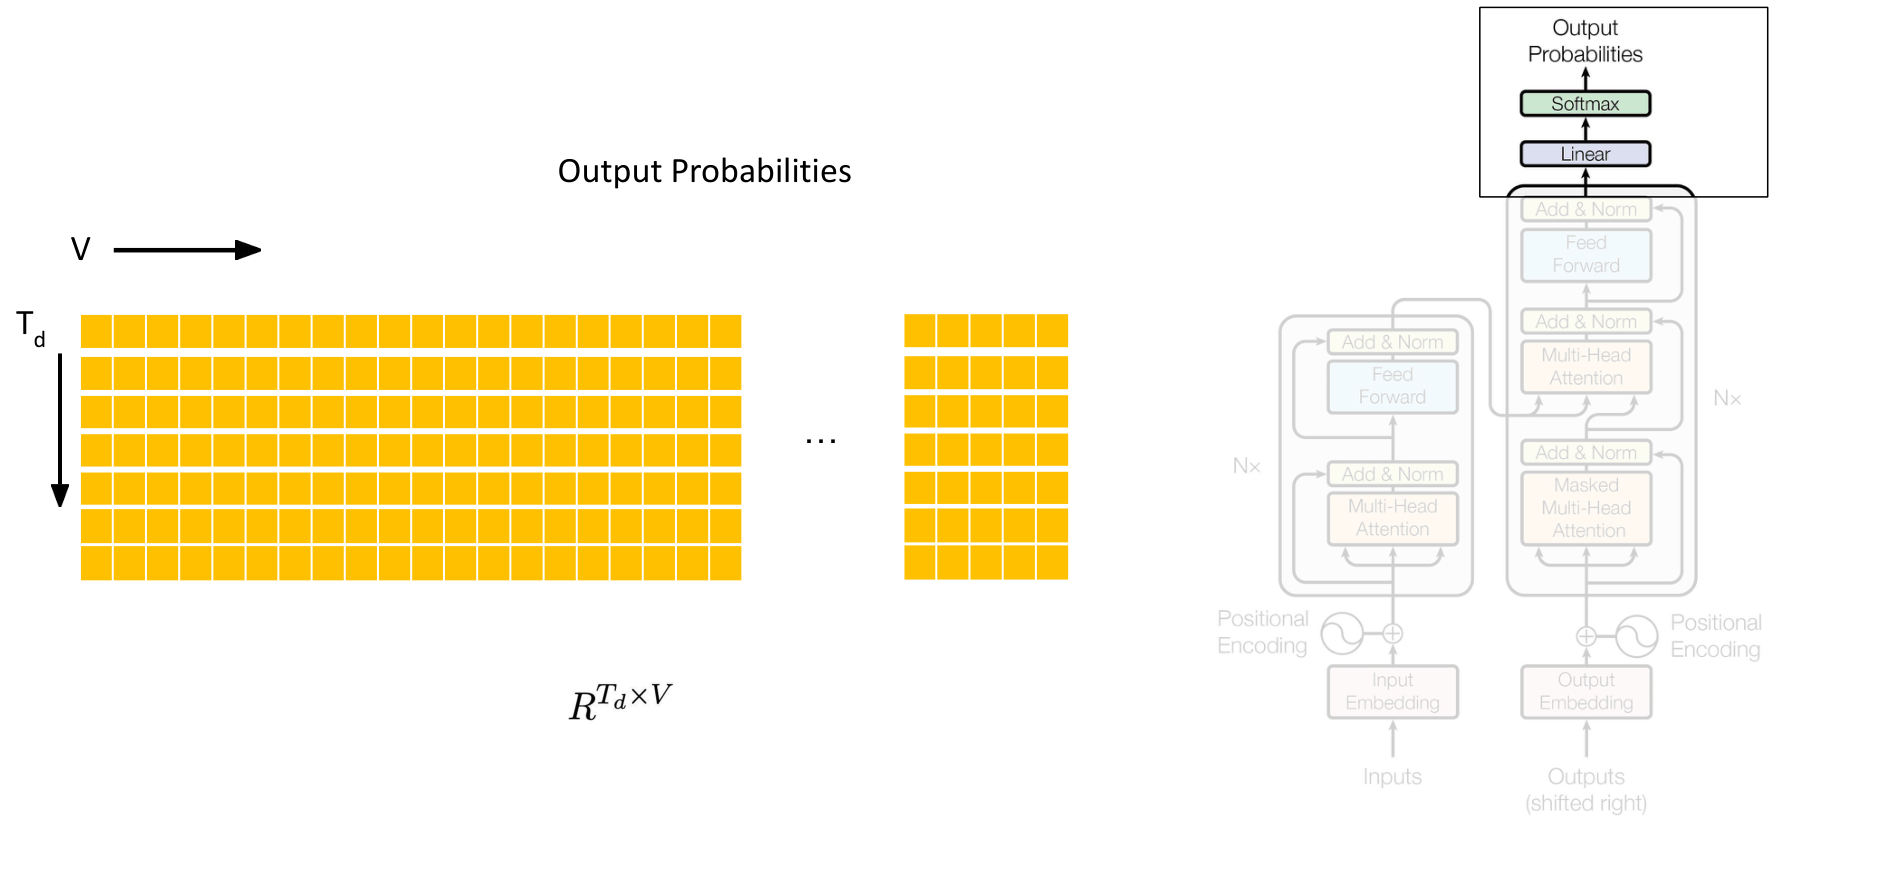
\includegraphics[width=0.8\paperwidth,height=0.8\paperheight,keepaspectratio]{images/introduction-to-transformers/transformer_output_probabilities_softmax_matrix.png}
\end{frame}

\begin{frame}{Transformers}
  \centering
  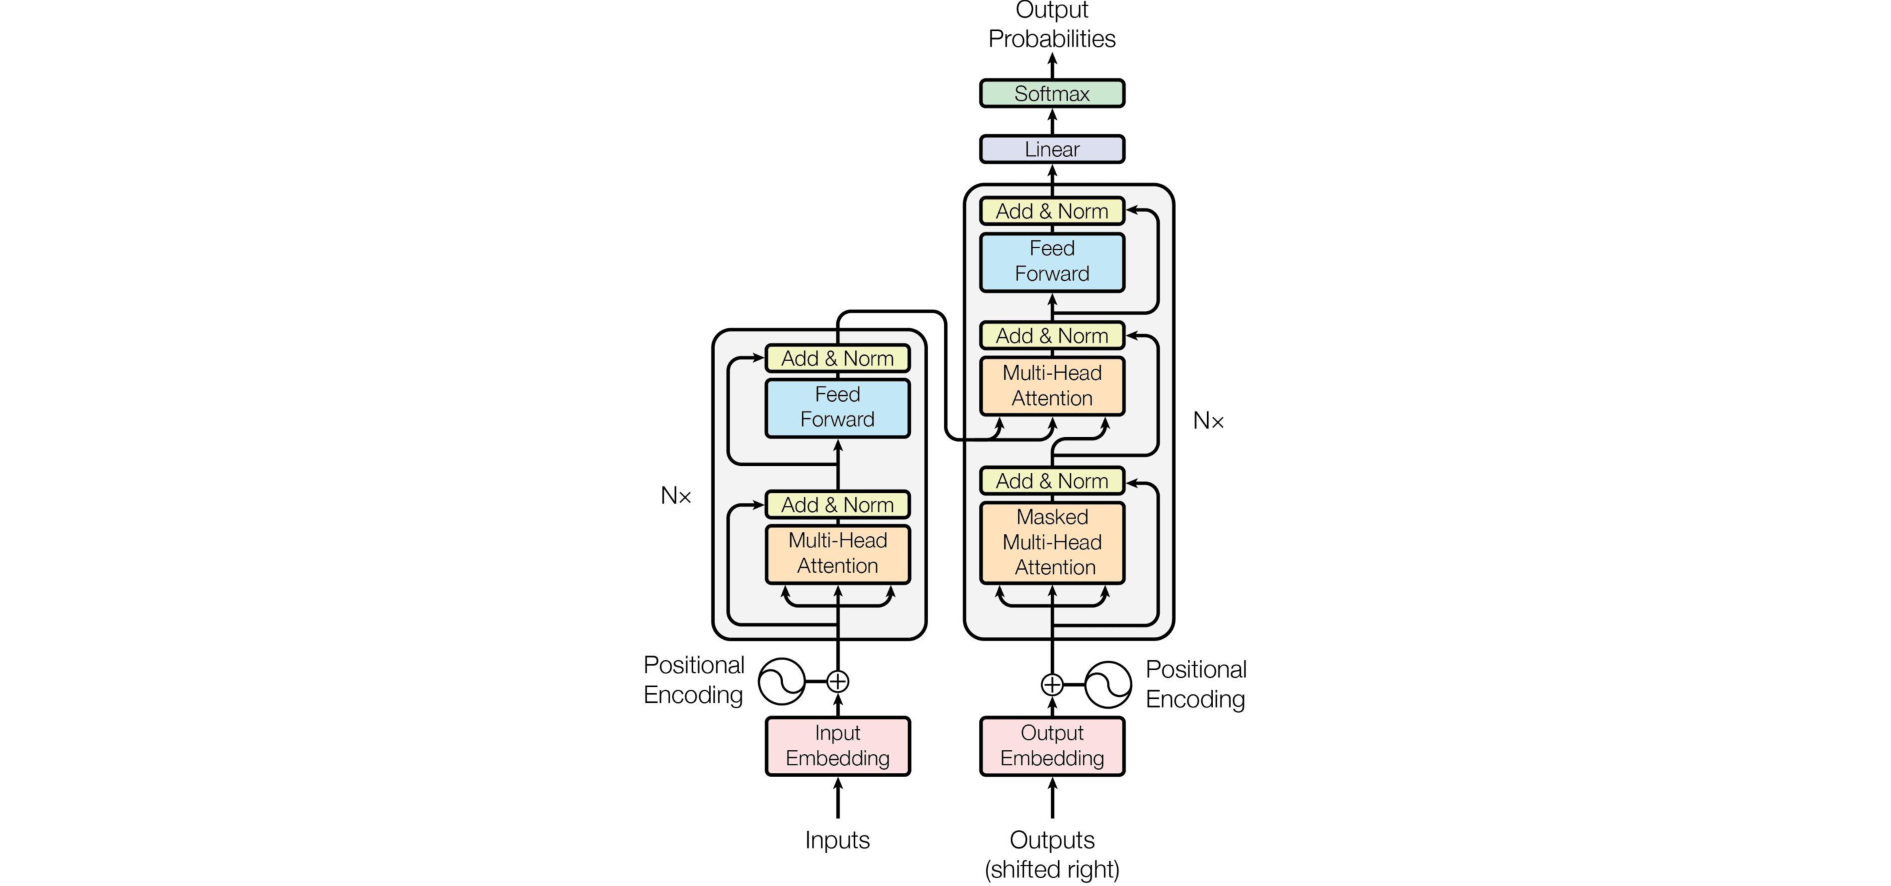
\includegraphics[width=0.9\paperwidth,height=0.9\paperheight,keepaspectratio]{images/introduction-to-transformers/transformer_full_encoder_decoder_architecture.png}
\end{frame}

\begin{frame}{Transformers}
  \centering
  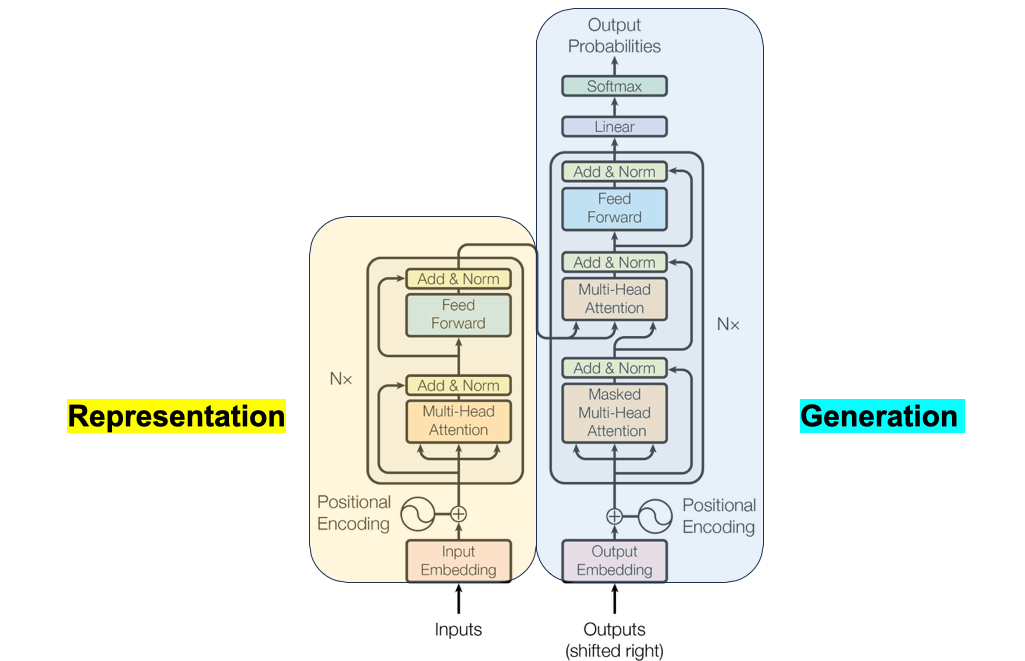
\includegraphics[width=0.8\paperwidth,height=0.8\paperheight,keepaspectratio]{images/introduction-to-transformers/transformer_representation_vs_generation_labeled.png}
\end{frame}

\begin{frame}{Transformers}
  \centering
  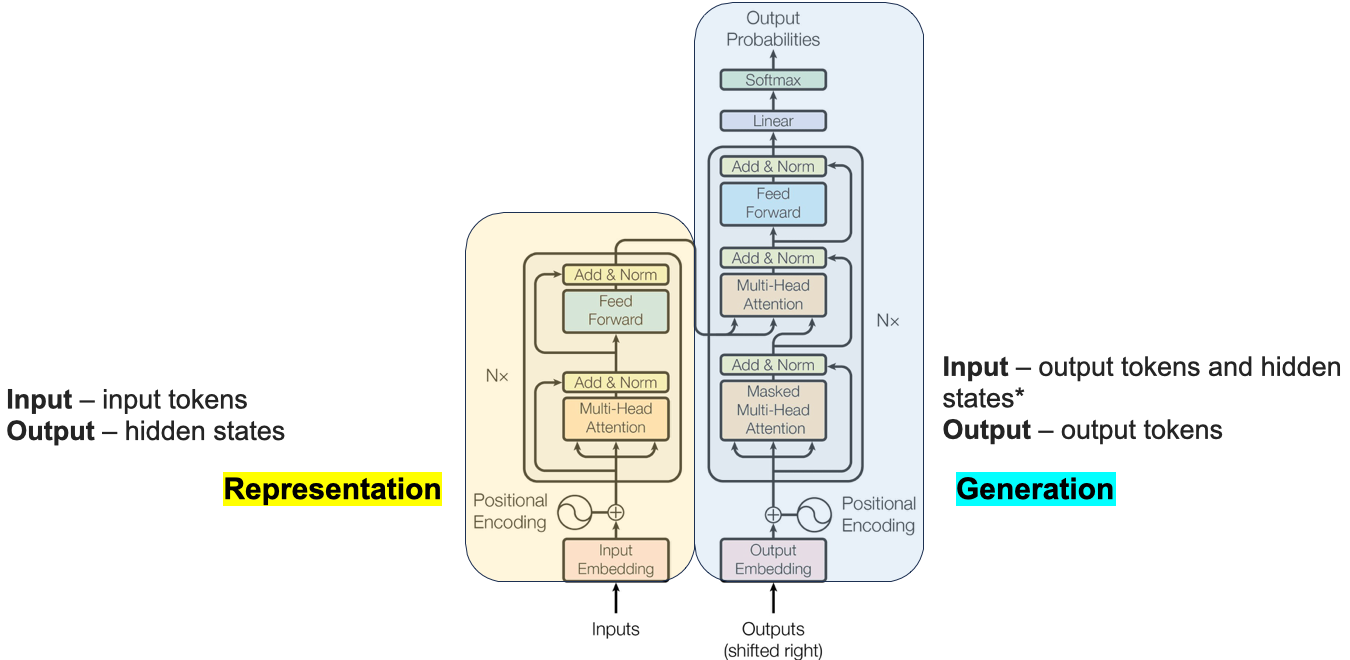
\includegraphics[width=0.9\paperwidth,height=0.9\paperheight,keepaspectratio]{images/introduction-to-transformers/transformer_encoder_decoder_input_output_definitions.png}
\end{frame}

\begin{frame}{Transformers}
  \centering
  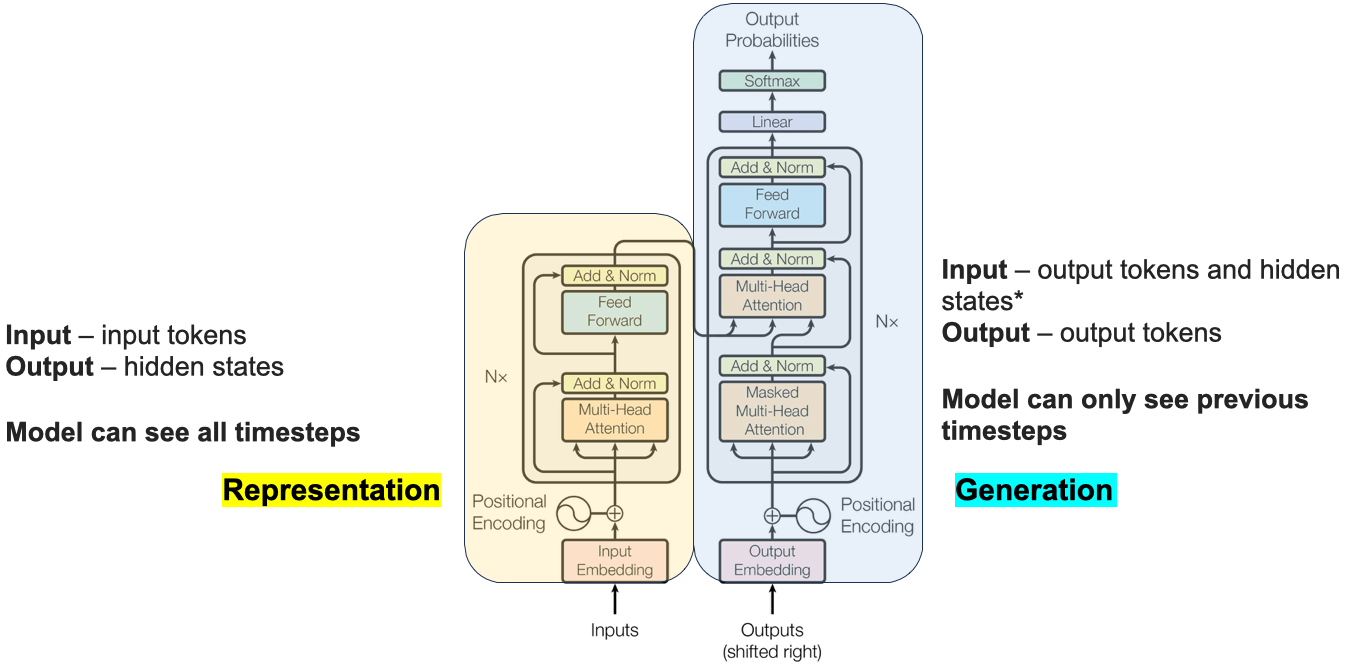
\includegraphics[width=0.8\paperwidth,height=0.8\paperheight,keepaspectratio]{images/introduction-to-transformers/transformer_encoder_all_timesteps_vs_decoder_previous_timesteps.png}
\end{frame}

\begin{frame}{Transformers}
  \centering
  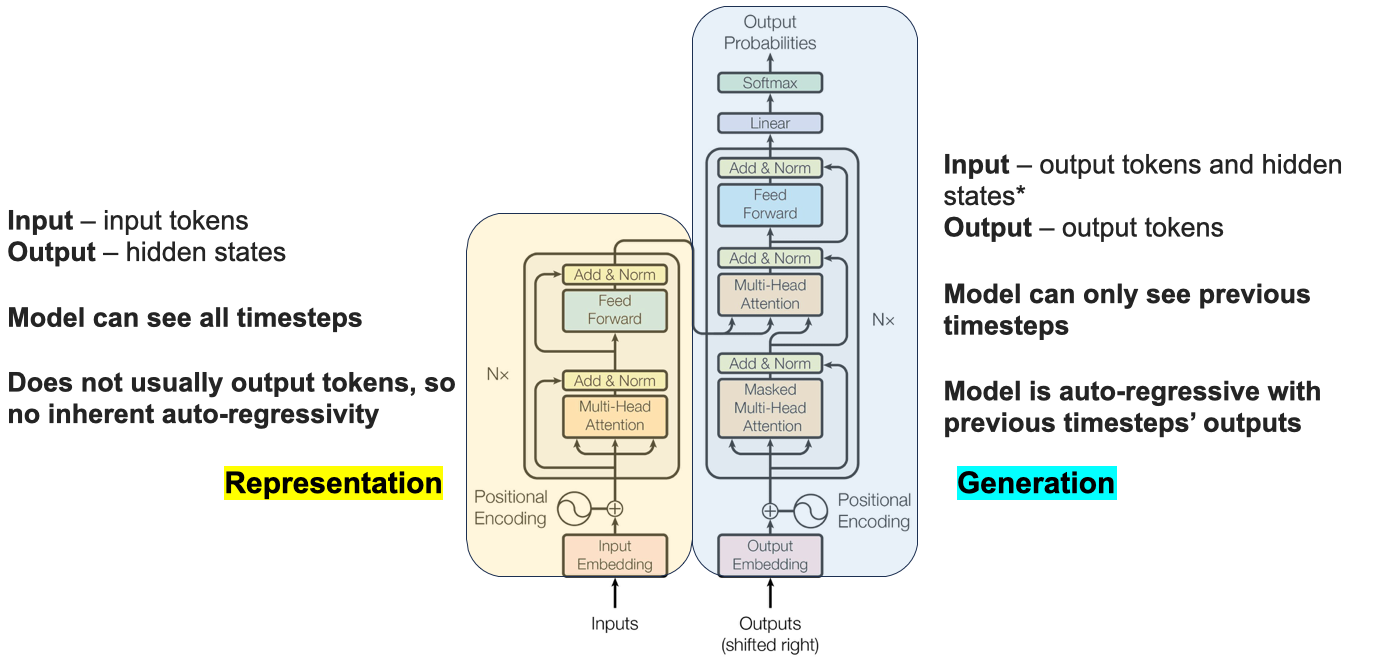
\includegraphics[width=0.8\paperwidth,height=0.8\paperheight,keepaspectratio]{images/introduction-to-transformers/transformer_encoder_no_autoregression_vs_decoder_autoregressive.png}
\end{frame}

\begin{frame}{Transformers}
  \centering
  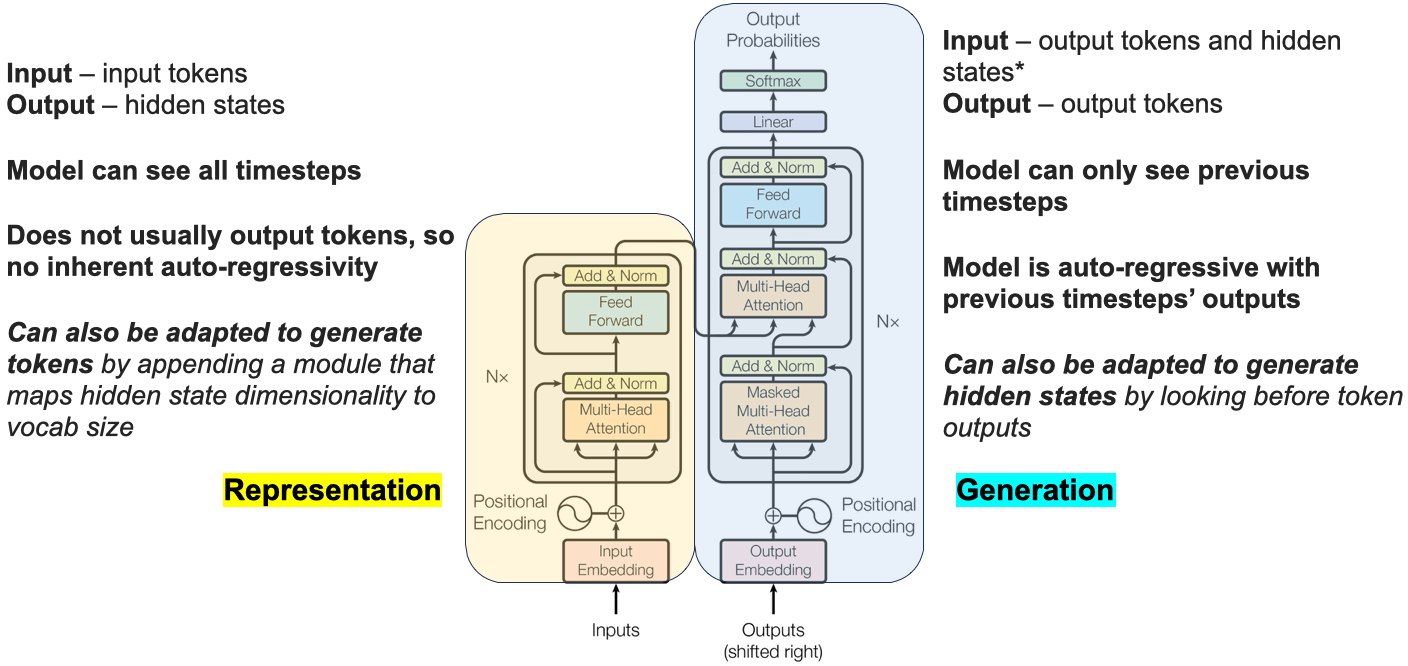
\includegraphics[width=0.8\paperwidth,height=0.8\paperheight,keepaspectratio]{images/introduction-to-transformers/transformer_encoder_decoder_adaptation_summary.png}
\end{frame}

